\documentclass{article}
\usepackage[utf8]{inputenc}
\usepackage{amsmath}
\usepackage{geometry}
\usepackage{listings}
\usepackage[T1]{fontenc}
\usepackage{fourier}
\usepackage{graphicx}
\usepackage{caption}
\usepackage{subcaption}
\usepackage{pythonhighlight}

\title{BIM3008-Assignment3 Report}
\author{Junyang Deng (120090791)}
\date{\today}
\geometry{left=1.5cm,right=1.5cm,top=2cm,bottom=2cm}

\begin{document} 
\maketitle
\section{Introduction}
Breast cancer is the most common type of cancer for females. 
One important task for researchers to improve the survival rate of BRCA patients is to identify the cancer stage and apply different treatment strategies. We can train a model to classify cancer stages using RNA-seq data from patient samples. In this project, I used support vector machine (SVM), random forest (RF), and k-nearest neighbor (KNN) to classify RNA-seq data. Then, 5-fold cross-validation is used to select the best hyperparameters for the model. Finally, we used the best model to predict the cancer stage of the test set.
\section{Procedure}
\subsection{Data Retrieval}
Data required for this project is retrieved from the UCSC Xena database. We used the FPKM normalized gene expression RNA-seq data %https://xenabrowser.net/datapages/?dataset=TCGA-BRCA.htseq_fpkm.tsv&host=https%3A%2F%2Fgdc.xenahubs.net&removeHub=https%3A%2F%2Fxena.treehouse.gi.ucsc.edu%3A443
and phenotype labels from the BRCA dataset. %https://xenabrowser.net/datapages/?dataset=TCGA-BRCA.GDC_phenotype.tsv&host=https%3A%2F%2Fgdc.xenahubs.net&removeHub=https%3A%2F%2Fxena.treehouse.gi.ucsc.edu%3A443
\subsection{Data Preprocessing}
Original reads data has $60483$ rows and $1218$ columns, each row is a gene and each column is a sample. The corresponding phenotype label table has $1284$ rows and $140$ columns. Each row represents a sample and each column represents a phenotype label. Only sample IDs and cancer stage diagnoses are used in this project, so the rest of columns are removed. Among the samples, \texttt{2} and \texttt{12} samples are removed because they have no labels and no diagnoses, respectively. 
Then, to make the classification task more realistic, we combined the substages of cancer. Originally, there are 13 diagnoses labels (including \texttt{not reported}). After combinding the substages, only 5 labels remain (See Table~\ref{table:label1} and \ref{table:label2}).
\begin{table}[tbhp]
\parbox{0.5\linewidth}{
    \centering
    \caption{Original cancer stage labels}
    \begin{tabular}{cccc}
        \hline
        Stage      & Number & Stage        & Number \\ \hline
        stage iia  & 415    & stage iv     & 22     \\
        stage iib  & 310    & stage x      & 13     \\
        stage iiia & 178    & not reported & 12     \\
        stage i    & 114    & stage ib     & 7      \\
        stage ia   & 94     & stage ii     & 6      \\
        stage iiic & 77     & stage iii    & 2      \\
        stage iiib & 32     &              &        \\ \hline
    \end{tabular}
    \label{table:label1}
}
\hfill
\parbox{0.5\linewidth}{
    \centering
    \caption{Cancer stage labels after processing}
    \begin{tabular}{ll}
        \hline
    Stage label & Number \\ \hline
    stage i     & 215    \\
    stage ii    & 731    \\
    stage iii   & 289    \\
    stage iv    & 22     \\
    stage x     & 13     \\ \hline
    \end{tabular}
    \label{table:label2}
}
\end{table}

Two dataframes needed to be merged before further analysis. Here, the \texttt{merge} function in pandas is used. Before merging, we first transposed the expression dataframe and changed the names of the \texttt{ID} columns in both dataframes into \texttt{sample\_ID}. The merged data frame has $1204$ rows and $60845$ columns.

After merging two datafremaes, samples are divided into train and test sets using the \texttt{train\_test\_split} function in \texttt{sklearn}. 30\% of data are randomly assign to test set.

\subsection{Model selection and cross-validation}
Three algorithms, support vector machine (SVM), random forest (RF) and k-nearest-neighbor (KNN) are used to solve this problem. All models used in this study are from \texttt{sklearn} (as shown in Table~\ref{table:algorithms}). 

\begin{table}[htbp]
    \centering
    \caption{Algorithms used in this study}
    \begin{tabular}{lll}
    \hline
    Algorithm & Class in sklearn & Key Parameters\\ \hline
SVM       & \texttt{sklearn.svm.svc}                         & gamma, kernel                                          \\
RF        & \texttt{sklearn.ensemble.RandomForestClassifier} & n\_estimators, max\_depth, min\_samples\_split, ... \\
KNN       & \texttt{sklearn.neighbors.KNeighborsClassifier}  & n\_neighbors                                     \\ \hline
    \end{tabular}
    \label{table:algorithms}
\end{table}
Baseline performance for all three models are shown in Figure~\ref{fig:svm}-\ref{fig:knn}.
\begin{figure}[htbp]
	\parbox{0.3\linewidth}{
        \centering
		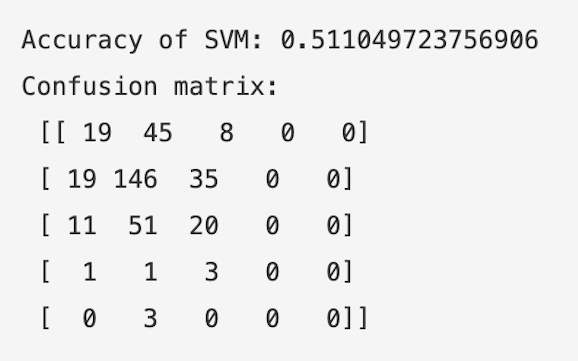
\includegraphics[width=\linewidth]{images/svm.png}
        \caption{}
        \label{fig:svm}
	}
	\hfill
	\parbox{0.3\linewidth}{\centering
		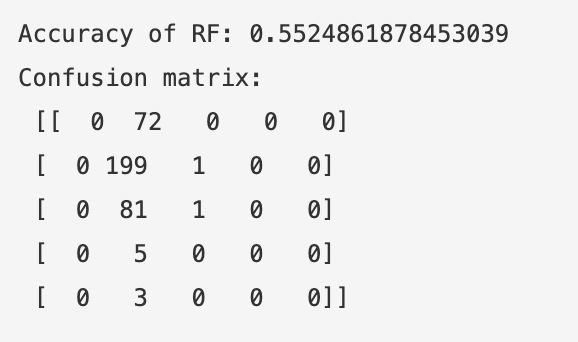
\includegraphics[width=\linewidth]{images/rf.png}
        \caption{}
	}
    \hfill
    \parbox{0.3\linewidth}{\centering
		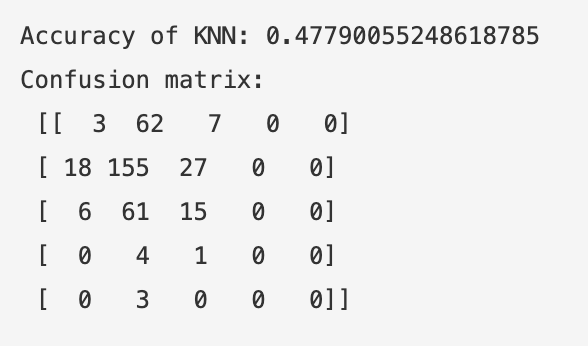
\includegraphics[width=\linewidth]{images/knn.png}
        \caption{}
        \label{fig:knn}
	}
\end{figure}
After obtaining the baseline performance, we conduct cross-validation to find the best hyperparameters. Class \texttt{sklearn.model\_selection.GridSearchCV} is to perform this process.
\begin{python}
# settings for SVM
svm_params = {
    'kernel':['linear', 'sigmoid', 'poly', 'rbf'],
    'gamma':['auto', 'scale'],
    }
grid1 = GridSearchCV(SVC(), svm_params, cv=3, verbose=3, n_jobs=-1)
# settings for RF
rf_params = {'bootstrap': [True, False],
              'max_depth': [5, 15, 50, 100, None],
              'max_features': [20, 50, 80],
              'min_samples_leaf': [1, 2, 4],
              'min_samples_split': [2, 5, 10],
              'n_estimators': [10, 100, 200]}
grid2 = GridSearchCV(RandomForestClassifier(), rf_params, cv=3, verbose=3, n_jobs=-1)
knn_params = {'n_neighbors':[5, 10, 20, 50, 100]}
# settings for KNN
grid3 = GridSearchCV(KNeighborsClassifier(), knn_params, cv=3, verbose=3, n_jobs=-1)
\end{python}
Results for cross-validation hyperparameter tuning can be access through \texttt{grid.best\_params\_}. The results are listed in Table~\ref{table:params}.
\begin{table}[htbp]
    \centering
    \caption{Best parameters}
    \begin{tabular}{lll}
    \hline
    Algorithm & Best parameters & Performance\\ \hline

    SVM       & \texttt{`gamma': `auto', `kernel': `sigmoid'} & 0.5524\\
    RF        & \texttt{`bootstrap': False, `max\_depth': 50, `max\_features': 50}, & 0.5414 \\
    &\texttt{`min\_samples\_leaf': 1, `min\_samples\_split': 5, `n\_estimators': 100}& \\
    KNN       & \texttt{`n\_neighbors': 50}    & 0.5497 \\ \hline
    \end{tabular}
    \label{table:params}
\end{table}
\subsection{Feature selection}
Apparently, 64000+ features are definitely too much, and most of them must be noise. To improve model performance, we can do feature selection to pick out important genes for the classification task. Two different approaches have been used in this study. One is to apply traditional feature selection methods. Another approach is to select features based on prior biology knowledge. These two approaches are elaborated in the following subsections.
\subsubsection{Select features based on correlation}
Genes with have constant expression level among different samples not only could not benefit stage classification, but also create noise for the task. Therefore, the first feature selection method we used is to set variance threshold for genes. The \texttt{sklearn.feature\_selection.VarianceThreshold} transformer is used to complete this job. We set the variance threshold to be 0.5. After transformation, $5685$ features (genes) were left. 

The second method is to choose features that are correlated with labels. Correlation is evaluated by chi-square. This idea is realized using the \texttt{sklearn.feature\_selection.SelectKBest} selector and the \texttt{sklearn.feature\_selection.chi2} method. We selected 566 features with highest chi-square scores. The number of features selected were decided by a p-value threshold (<0.01).

\subsubsection{Select features based on prior biology knowledge}
Since we are predicting breast cancer stages based on gene expression profile, knowing which gene is important for stage classification will be very helpful. 109 genes were selected from literature \cite{breastcancer}, including some growth factors like PDGF and growth-related pathways (MAPK, PI3K-Akt, ...) (The full list of selected genes are in the \texttt{list\_of\_genes2.txt} file). 

\subsection{Result}
Model performance (evaluate by accuracy) using three models and is calculated on original features and three sets of newly selected features (Table~\ref{table:performance}). Sadly, any of feature selection methods cannot yield significantly better result. For a 5-class classification problem, an accuracy of 50\% seems acceptable. However, the best accuracy (0.5552) is obtained when a model classified almost all samples into the stage II (by random forest classifier, after feature selection). The same situation persists even when the problem was changed into a binary classification problem. This means that current models don't have the ability to distinguish stage II and other stages. More information, such as histological image data and proteomic data, should be intergrated to make a better result.
\begin{table}[htbp]
    \centering
    \caption{Performance of three models on different features}
    \begin{tabular}{lllll}
        \hline
        Model & Original data  & Variance threshold & Chi-square    & Prior knowledge \\
              & k=60428        & k=5675             & k=566         & k=109           \\ \hline
        SVM   & 0.5524 (33.5s) & 0.5497 (0.4s)      & 0.5497 (0.2s) & 0.5552 (0.2s)   \\
        RF    & 0.5525 (13.9s) & 0.5497 (0.2s)      & 0.5525 (1.1s) & 0.5552   (0.6s) \\
        KNN   & 0.4779 (1.8s)  & 0.5234 (0.6s)      & 0.5328 (0.8)  & 0.5497 (0.4s)   \\ \hline
    \end{tabular}
    \label{table:performance}
\end{table}


\bibliographystyle{unsrt}
\bibliography{ref}
\end{document}
